% !TEX root = ../main.tex
\section{Usability Testing of the Survey}\label{sec:usabilitytestingsurvey}

  The usability of the survey was being tested before starting collecting data for different purposes. {\it First}, when sending out the survey, there is no much room for changing the layout and content of the survey. The layout and content should be looking the same for all respondents. A change in the formulation or a change in the layout can cause respondents to interpret a question differently. {\it Second}, the survey is in a non-controlled environment, meaning that knowing who the participants are and where they are from are not known. The questions and layout needs to be created as universal and as intuitive as possible. The questions, the flow, and the graphical elements should be intuitive across different countries and cultures. 

  The usability testing is divided in two main parts: usability testing in a controlled environment and usability testing in an uncontrolled environment. Beside the specific usability tests performed, it has also been performed testing on the selected icons as well as the wireframes created in the preliminary work /cite{forprosjekt}. A summary of usability test of the icons will be provided in this section. The usability test performed on the wireframes provided in Appendix \ref{ap:wireframes} resulted in the first implemented version being tested in this study. 

  \subsection{Testing the Icons}\label{sec:usabilityicontest}
  As a described in the requirements, respondents should be able to understand and interpret the questions correctly regardless of the language spoken. As a cause of the requirement, icons were chosen to be used instead of using text. If the icons should work as intended, the icons should be properly tested. 

  When testing the icons, the goal is to get the participants in the test to interpret what being asked for by only looking at the icons. In other words, the respondents had to guess the formulation of the question by looking at the icons. The test was performed by using all the icons selected for the survey. The test were performed on 12 students; 5 female and 7 male students.

  All the respondents managed to guess the questions asked for most of the questions to some extent. Each attempt had some variations but were considered to be correctly enough for passing. When the icons are used in the survey, the question is provided. Some of the participants had some problem interpreting the different locking mechanisms in the screen asking for the locking mechanism currently in use, especially the {\it slide-to-unlock}. Some of the questions used a question using the alternatives with a green check mark, and a red cross mark indicating the answer no. For the check mark and the cross, the respondents were asked to interpret thir purpose. All of the respondents either categorized the icons as "agree/disagree" or "yes/no".

  \clearpage
  \subsection{Testing the Survey in a Controlled Environment}
  To perform a usability test in a controlled environment, meaning that one responsable person have set up an environment being observable, as well as that person being present. The test was conducted in a quiet meeting room by testing 10 students, 5 boys and 5 girls from the Norwegian University of Science and Technology. The participants had different background, but the majority were studying Computer Science.

  To ensure the test was being conducted in an environment close to how the survey works, they brought their own device and they were not being told much about the research. All the participants got the same introduction and instructions of how the test worked:

      \begin{enumerate}
        \item The participant were asked to speak aloud during the test and tell what they were thinking and reason about their choices.
        \item The participants were told that the test was not testing their ability to finish the test.
        \item The participants were explained that they could quit the test if they felt uncomfortable
      \end{enumerate}

  After giving an introduction to the test, the participant got the URL to the survey, and they were asked to start whenever they felt ready. In the list below there is listed comments from the participants that was stated during the test. The following statements listed below were useful statements from the persons testing the application. The statements are either useful comments provided during the test or observation might causing a need for doing changes in the application:

  {\it "How do I get back if I press a wrong answer?"}\\ 
  One of the persons asked how it was possible navigating back to a previous question if a wrong answer were being selected. The participant expected a button working similar to an undo button for being able to undo a wrong answer.

  {\it "Too many icons on the screen for representing different screen locks"}\\ The person did find it confusing with all the icons representing the different screen locks. The participant also found it hard to interpret and select the intended screen lock. As this caused problems, the respondent would like this being presented in an another way, hence eliminate the ambiguity and confusing visualization by using too many icons. One suggestion was to add a description to each of the icons or to replace the icons using a list with only text.

  {\it "I need to choose a pattern that is hard to guess for the banking account!"}\\ 
  Most of the participants used more time creating a pattern for a banking account than for the other patterns. Some of them also commented that they did spend more time creating this than the other patterns because they felt the need for creating protecting their banking account more than for the other types. It was also noticeable that the participants used more time thinking before creating the pattern for the banking application. Some of the respondents also acknowledged that they used a pattern for smartphone that they had used or were currently using. 

  {\it "Do I choose the size of my hand based on my gender?"}\\ 
  Four of the participants was uncertain on how to categorize the size of their hand. Some of the participants commented on whether they selected their hand size based on their gender or categorizing the hand based on unisex sizes.

  {\it "Tody, my smartphone would probably be categorized as a medium smartphone"}\\
  The question is by definition subjective, but there is no easy for asking this differently. The provided answer might depend on the person's technical experiences with smartphones. Today, most of the smartphones would be categorized as a medium size, while older smartphones would probably fall into the category small size. For avoiding any ambiguities, an new solution should be found ensuring quality in the data collected.

  {\it "I expected to type the pattern after creating the pattern"}\\ 
  One of the participants expected to be asked to retype the pattern. The respondent did not have any preferences of when the patterns should being asked to be retyped. Two suggestions was to either copy the pattern creation process of Android or asking the respondents to recreate the patterns at the end of the survey.

  {\it "I do read from left to right, but I do also read lines from top to bottom."}\\ 
  Three of the participants either was unsure what the question asked about or did not understand the icons used. The view should be redesigned to avoid any ambiguities in the presentation. One provided from the respondents was to used examples next to the icons. 

  {\it "The last question about my experience with IT and security took a while to understand."}\\ 
  The question was long and complex. Many of the participants used a long time interpreting the question and some of them asked me during the test if they had understood the question correctly. The formulation should be changed for avoiding such situation.

  \subsection{Testing the Survey in an Uncontrolled Environment}
  Observation of incoming data is not a typical usability test but is rather a quality check to see whether the collected data is reasonable. When sending out the survey without being present, it is important to validate the incoming data to see if any respondents have any problems related to completing the survey or interpret the questions. As a test, the survey was first distributed to a small group of selected people from Norway (ISO country code 'NO').

  When looking through the data, it was observed that one person were registered rare and small country in Africa with the ISO country code starting with 'N'. It is reasonable that this was a typing error or something wrong with the component used in the question. The component used in the question was a third party dropdown list with a flag icon for each country. It were observed that the component used were using a long time loading the flag, hence lagging while the respondents interacted with the component. The component should be changed and optimized to avoid such situation. 

  The majority of the people asked to participate in an early release were living in Scandinavia, hence having a reading and writing direction from left to right. When looking through the collected data, 2 out of  25 respondents had selected otherwise. Based on statistics, there should only be persons with reading and writing direction from left to right. One assumption is that the icons used are being ambigiuos, hence interpreted wrong. 

  Besides looking at the data, I received feedback by email from some respondents answering the survey for testing purposes. They commented that the dropdown were lagging, as well as being confused when selecting the screen lock they were currently using. 

  \subsection{Changes Made to the Survey}
  Before distributing the survey there were conducted two types of tests providing useful insight of how the users experienced the application. The tests were crucial because of the high need for high-quality data collected from the survey. Any ambiguities or errors causing bias in the data are not wanted. This section will provide information on all changes made to the application as a result of the observations and the feedback from the tests.

    \subsubsection*{1) Country dropdown}
    In both tests, there were many participants that unintentionally selected the wrong country because the dropdown component lagged. The component used had a flag attached to the country name that used many resources for loading, causing the users experiencing the component to be slow. The component was changed, and the flag icons were removed. Figure \ref{fig:change-country-old} and \ref{fig:change-country-new} are showing the old and the new version of the country component, respectivley.

      \begin{figure}[H]
        \centering
        \subfigure[Old view]{
          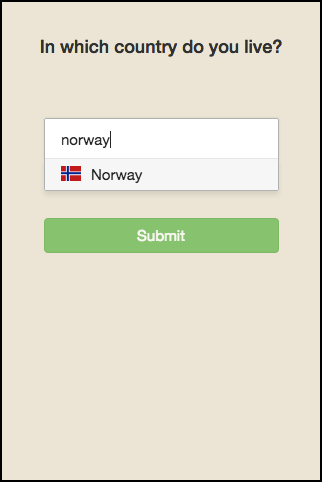
\includegraphics[scale=0.34]{pics/survey/country-old}
          \label{fig:change-country-old}
        }
        \subfigure[Final view after changes]{
          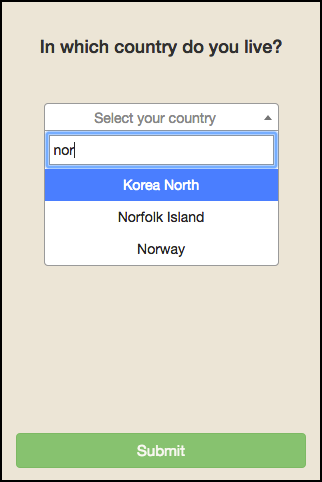
\includegraphics[scale=0.34]{pics/survey/country2}
          \label{fig:change-country-new}
        }
        \caption{Changes in country selection view}
        \label{fig:change-country}
      \end{figure}

    \subsubsection*{2) Experience question}
    The question was rather complicated and hard to read. The question was changed from "Do you work with or study/studied IT and/or security full time?" to "Do you have a background in IT/Security?".

    \subsubsection*{3) Reading and writing direction}
    The first version of the survey just listed three different icons of arrows indicating the reading and writing direction, but it seemed that people misinterpreted the icons. This view was changed by adding a description next to the arrow to remove any misinterpretations of the icons. The old and the new presentation of the question are shown in Figure \ref{fig:change-readwrite-old} and \ref{fig:change-readwrite-new}, respectively.

      \begin{figure}[H]
        \centering
        \subfigure[Old view]{
          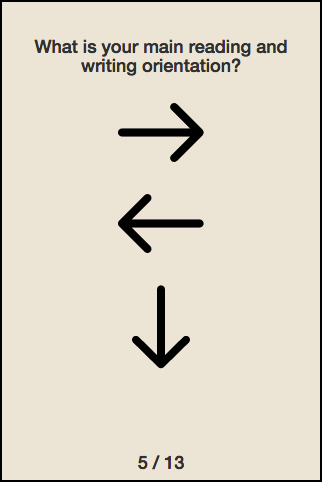
\includegraphics[scale=0.34]{pics/survey/reading-old}
          \label{fig:change-readwrite-old}
        }
        \subfigure[Final view after changes]{
          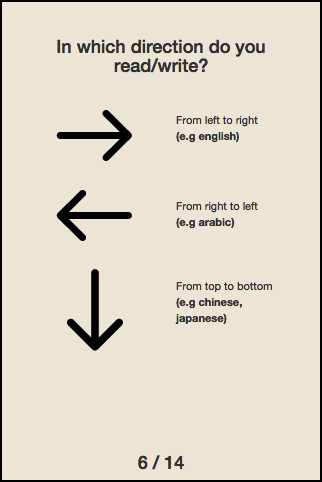
\includegraphics[scale=0.34]{pics/survey/reading}
          \label{fig:change-readwrite-new}
        }
        \caption{Changes in reading/writing direction view}
        \label{fig:change-readwrite}
      \end{figure}

    \subsubsection*{4) Apply time used into creation of patterns}
    It was observed that some of the participants in the usability test in the controlled environment was spending more time creating the pattern for banking account. During the test, it was not easy to track the time used on different tasks, but this can be implemented in the application for observing the time used for creating a pattern of a spesific type.
    The observation from the test was that some of the participants took their eyes off the screen thinking harder about the pattern they wanted to create for the banking account. In this test, I was present and could observe such situations, but are not possible when distributing the survey. Such time frame can also be used in the analysis. An example of use could be to eliminate dishonest attempts causing bias in the data. 
  

    \subsubsection*{5) Selection of screenlock}
    The first version of the view had a list of all the screen locks that are provided on the majority of the smartphones. Based on feedback, the participants found it confusing to select the correct screen lock for several reasons.{\it First}, some of the participants did not understand all the icons used. {\it Second}, it was observed that some of the users did not interpret all the alternatives and selected the first matching alternative. {\it Third}, it seems that some had a screen lock that could be categorized as several of the presented icons, making it hard to pick the correct one. The new version of the view replaced all the icons with a drop-down listing all the alternatives. When the user selects a screen lock, an image or description appears below the dropdown, giving an extra layer of confirmation of the selected screen lock. The alternative "PIN" was also changed from "PIN" to "PIN (4-digits)" for eliminate any ambiguities for those using more than four digits. Figure \ref{fig:change-screenlock-old} and \ref{fig:change-screenlock-new} are the old view and the new view, respectively.
    
      \begin{figure}[H]
        \centering
        \subfigure[Old view]{
          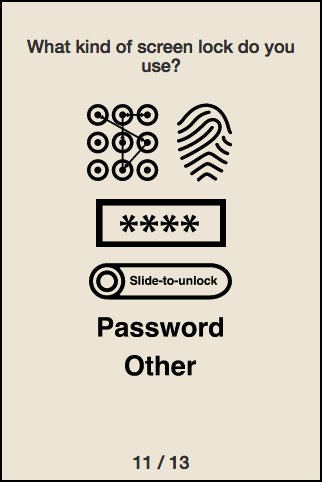
\includegraphics[scale=0.34]{pics/survey/screenlock-old}
          \label{fig:change-screenlock-old}
        }
        \subfigure[Final view after changes]{
          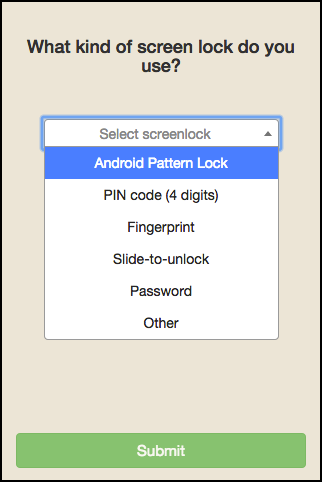
\includegraphics[scale=0.34]{pics/survey/screenlock2}
        }
        \caption{Changes in screenlock selection view}
        \label{fig:change-screenlock-new}
      \end{figure}

    \subsubsection*{6) Changing handsize question}
    Based on feedback from the test conducted in the controlled environment, the participants did not know what to compare their hand size to. The size selected depended on whether they compared themselves to their gender or not. For being consistent, the question explicitly stated in the question that the user should select their size based on their gender. 

    \subsubsection*{7) Adding pattern retype}
    During the tests, it was received feedback that many of the participants expected to be asked to retype their selected patterns. Two suggestions from the respondents were to copy the process used on Android devices or asking respondents to retype in the end of the survey. It is not desired to ask users to retype their patterns at the end of the survey because such situation can make respondents feeling if not being able to remember the pattern. As stated in the requirements, respondents should not leave the survey with a bad experience. If asking the respondents to retype the pattern at the end of the survey, this should be clearly stated before creating the patterns. By stating that the users should remember the patterns for being able to complete the survey could cause respondents feeling uncomfortable or even cause the respondents to leave the survey. The best solution was to copy the same process that Android are using.

    \subsubsection*{8) Collecting screen pixels of screen used}
    By observing the participants in the first test, it was observed that the selected choice in patterns was different from person to person. Since this question is a subjective meaning of the person answering, an extra layer of information is applied to the dataset by saving the pixels width and height of the screen. One problem with pixels size of a mobile screen is that they do not match the physical size of the screen. The pixels could still provide information for being able to categorize the size correctly by comparing the OS and pixels to the respondents answer.

    \subsubsection*{9) Shuffle the ordering of the patterns}
    One concern with asking the users to create the patterns in a predefines order as discussed until now, respondents might be influenced by the order of the patterns. 

    To be sure that the ordering is not introducing bias, a method named {\it Latin Square} can be used. A Latin Square is a table filled with n different symbols in such a way that each symbol occurs exactly once in each row and exactly once in each column. Instead of using three different orderings, all possible combinations of the three pattern types will be used. This results in 6 different ways of ordering the patterns.

    By using the Latin Square, it ensures that the ordering do not impact the respondent's choice of patterns. Or in other words, the data can be validated afterwards to see if the ordering have affected the collected data. In practice, respondents will create the same patterns, but in a different order. 

  \clearpage
  \section{Ethical Considerations}\label{sec:ethics}
    
    My research is performed by collecting demographics and other information about the respondents and the devices used. The data are not by definition considered to be sensitive information, in other words, the information can not be linked back to the respondent. It is still important to evaluate the work being done for avoiding conducting research not considered being ethical. As this research are collecting user-selected patterns, a set of countermeasures have been implemented for ensuring anonymity of the respondents. 

    Before the survey starts, the respondents are informed about the purpose of the research and how their contributed data will be managed. Respondents are also advised that they have the right to leave the survey whenever wanted. The questionnaire should be entirely anonymous, and the identity and location of the respondent should not be possible to track back to the respondent. As the selected sampling technique supports, a list of respondents is not kept in any form as the respondents participate voluntarily if receiving the survey. Other measures applied are turning off the logging of the IP addresses on the server side. The application are made by the researchers and for this research in particular. Therefore, no third part is included or have access to the data, making it possible to ensure anonymity. 

    Before collecting data, it is required to get an allowance for collecting data from the {\it NSD}, in Norwegian called {\it Personvernombudet for forskning} \cite{personvernombud}. The NSD is the privacy ombudsman for approximately 150 research and educational institutions in Norway, where NTNU is one of them. The research was reviewed and accepted by the supervisor of this project and the NSD contact person from NTNU. 

